\chapter{Completeness}

In this chapter,
we're going to meet some important results about the powers and limitations of first-order logic.
Our starting point is the completeness theorem,
which shows that there is a mechanical way to check for first-order entailment.
We'll see that this positive result is tightly connected to some negative results:
the compactness theorem and the Löwenheim-Skolem theorems.
These results concern the \emph{size} of models,
by which we mean the size of their domain.
To fully appreciate their implications,
I'll begin with some background about the sizes of sets,
which will be needed in later chapters anyway.

\section{Cardinalities}\label{sec:cardinalities}

$\{$ Athens $\}$ is a set with a one member:
the city Athens.
We say that $\{$ Athens $\}$ has size 1.
$\{$ Athens, Berlin $\}$ has size 2.
$\{$ Athens, Berlin, Cairo $\}$ has size 3.
And so on.
It seems straightforward.
But now consider the set $\mathbb{N}$ of natural numbers 0, 1, 2, 3, \ldots.
What is its size?

The official set-theoretic term for the size of a set is \textit{cardinality}.
So $\{$ Athens, Berlin, Cairo $\}$ has cardinality 3.
Finite sets have a finite cardinalities, which are natural numbers.
But infinite sets also have a cardinality.
These aren't natural numbers,
but numbers of a more general sort,
called \emph{cardinals}.
The infinite cardinals are also known as the \emph{alephs},
because they are conventionally written using the Hebrew letter `$\aleph$' (``aleph'').
For example,
the cardinality of $\mathbb{N}$ is called `$\aleph_0$'.
This is the smallest infinite cardinal.
The next larger one is $\aleph_1$,
followed by $\aleph_2$, and so on.

% You may be puzzled what sort of things the alephs are.
% I'll give an answer in the next chapter.
% But note that it is equally unclear what sort of thing the natural numbers are.
% The more important question is how the alephs behave.
How do we determine the cardinality of an infinite set?
The crucial idea goes back to Galileo and Hume,
but was only fully developed by Georg Cantor in the 19th century.
Following Galileo and Hume,
Cantor stipulates that
two sets have the same cardinality iff there is a one-to-one correspondence between their members.

To make this precise, we define the notion of a one-to-one correspondence, or bijection.

\begin{definition}{}{bijection}
  A function $f$ from a set $A$ to a set $B$ is a \emph{bijection}
  if it satisfies the following two conditions.
  \begin{enumerate*}
    \item[(i)] For every $x, y \in A$, if $f(x) = f(y)$ then $x = y$. (Injectivity)
    \item[(ii)] For every $b \in B$ there is some $a \in A$ such that $f(a) = b$. (Surjectivity)
  \end{enumerate*}
\end{definition}

Intuitively, a bijection pairs up each element of $A$ with exactly one element of $B$,
and vice versa,
so that every element of either set gets a unique partner.
As a shorthand,
we say that sets $A$ and $B$ are \emph{equinumerous} if there is a bijection from $A$ to $B$.
(In this case, there is always also a bijection from $B$ to $A$.)

The Galileo-Hume-Cantor principle now says that
\emph{two sets have the same cardinality iff they are equinumerous}.
Obviously,
no finite set of numbers is equinumerous with $\mathbb{N}$.
So $\mathbb{N}$ has an infinite cardinality.
We define `$\aleph_0$' to name this cardinality.
Using the Galileo-Hume-Cantor principle,
we can determine,
for any other set,
whether it also has cardinality $\aleph_0$.

Consider,
for example,
the set of odd numbers $1, 3, 5, 7, \ldots$.
The following function $f$ is a bijection from $\mathbb{N}$ to the set of odd numbers:
\[
  f(n) = 2n + 1.
\]
The function maps 0 to 1, 1 to 3, 2 to 5, and so on.
Every natural number is mapped to a unique odd number,
and no odd number is left unmapped.
So the set of odd numbers also has cardinality $\aleph_0$.

Galileo found this paradoxical:
how can there be as many odd numbers as natural numbers,
given that the odd numbers are a proper subset of the natural numbers?
Never mind,
said Cantor:
the resulting theory of cardinalities is consistent and mathematically fruitful,
even if it may initially seem strange.

Sets that are equinumerous with $\mathbb{N}$ are also called \emph{countably infinite} or \emph{denumerable}.
A set is \emph{countable} if it is either finite or countably infinite.
The word `countable' alludes to the fact that
a bijection between $\mathbb{N}$ and another set
effectively assigns a ``counter'' to each member of the set.
For example,
the above bijection between $\mathbb{N}$ and the odd numbers
assigns the counter 0 to 1, 1 to 3, 2 to 5, and so on.

\begin{exercise}
  Show that (a) the set of even natural numbers and (b) the set of integers $\ldots, -2, -1, 0, 1, 2, \ldots$ are both countably infinite.
\end{exercise}

% The set of integers $\mathbb{Z} = \{\ldots, -2, -1, 0, 1, 2, \ldots\}$ is also countably infinite.
% We can establish a bijection between $\mathbb{N}$ and $\mathbb{Z}$ by mapping:
% \begin{align*}
% 0 &\mapsto 0 \\
% 1 &\mapsto 1 \\
% 2 &\mapsto -1 \\
% 3 &\mapsto 2 \\
% 4 &\mapsto -2 \\
% 5 &\mapsto 3 \\
% &\vdots
% \end{align*}
% In general, we map even numbers $2n$ to positive integers $n$, and odd numbers $2n+1$ to negative integers $-n$.

% As the example illustrates,
% we can conceptualize a mapping from $\mathbb{N}$ to some set $S$ as a \emph{list}
% of the members of $S$.
% If we allow lists with repetitions,
% we can say that a set is countable iff its members can be put on an infinite list,
% each item of which has as ``index'' a natural number.

Are there any \emph{uncountable} sets?
We might suspect that the set of \emph{pairs} of natural numbers is uncountable.
But not so.
Cantor's \emph{zig-zag method} shows that
there is a bijection between $\mathbb{N}$ and the set of pairs of natural numbers.
We begin by arranging all pairs of natural numbers in a two-dimensional grid.
%
\begin{center}
  % ----------------------------  LAYERS  ---------------------------------
\pgfdeclarelayer{bg}
\pgfsetlayers{bg,main}        % bg drawn first (→ behind the grid)
% -----------------------------------------------------------------------

\begin{tikzpicture}[>=Stealth,
  every node/.style={font=\small},
  cell/.style={draw,minimum size=1cm},
  zig/.style ={orange!60,very thick,
               -{Stealth[length=3mm,width=3mm]},
               shorten >=5pt,shorten <=5pt}]

\def\N{4}                      % explicit indices 0…4 (→ 5×5 visible block)
\def\NN{\numexpr\N+1\relax}    % position of dotted row/column

% --------------------------  GRID + LABELS  ----------------------------
\foreach \i in {0,...,\NN}{%
  \foreach \j in {0,...,\NN}{%
    \coordinate (p) at (\j,-\i);
    \node[cell] (c\i\j) at (p) {};
    % what goes into the cell?
    \ifnum\i=\NN                     % last (dotted) row
        \ifnum\j=\NN
            \node at (p) {$\ddots$};
        \else
            \node at (p) {$\vdots$};
        \fi
    \else
        \ifnum\j=\NN                 % last (dotted) column
            \node at (p) {$\cdots$};
        \else                        % ordinary ordered pair
            \node at (p) {(\i,\j)};
        \fi
    \fi
  }%
}
% row and column headers
\foreach \i in {0,...,\N}{ \node at (-0.7,-\i) {\i}; }
\node at (-0.7,-\NN) {$\vdots$};
\foreach \j in {0,...,\N}{ \node at (\j,0.7) {\j}; }
\node at (\NN,0.7) {$\cdots$};

% -------------------------  CANTOR PATH  -------------------------------
\begin{pgfonlayer}{bg}
  \coordinate (prev) at (c00.center);  % starting point (0,0)

  % start with diagonal 1 – diagonal 0 would be only (0,0)
  \foreach \s in {1,...,\N}{%
     \ifodd\s                         % odd diagonal : NE direction
        \foreach \k in {0,...,\s}{%
           \pgfmathtruncatemacro\a{\k}
           \pgfmathtruncatemacro\b{\s-\k}
           \draw[zig] (prev) -- (c\a\b.center);
           \coordinate (prev) at (c\a\b.center);
        }%
     \else                            % even diagonal : SW direction
        \foreach \k in {0,...,\s}{%
           \pgfmathtruncatemacro\a{\s-\k}
           \pgfmathtruncatemacro\b{\k}
           \draw[zig] (prev) -- (c\a\b.center);
           \coordinate (prev) at (c\a\b.center);
        }%
     \fi
  }%
\end{pgfonlayer}
\end{tikzpicture}

\end{center}
%
We then define a path through this grid that visits each cell exactly once.
The orange arrows indicate that path.
It effectively enumerates all pairs $\t{x, y}$,
starting with $\t{0,0}$,
followed by $\t{0,1}$, $\t{1,0}$, $\t{2,0}$, $\t{1,1}$, $\t{0,2}$, and so on.
The enumeration amounts to a lists of all the pairs.
We get a bijection to $\mathbb{N}$ by assigning to each pair
its position in the list \t{starting with position 0}.
Thus $\t{0,0}$ is mapped to 0,
$\t{0,1}$ to 1,
$\t{1,0}$ to 2,
and so forth.

(We can find a formula for this bijection.
As we follow the arrow,
the pairs \emph{before} any given pair $(x,y)$ comprise
all the pairs on the left-to-top diagonals before $(x,y)$,
which have 1, 2, 3, etc. pairs,
plus the $y$ pairs on the diagonal containing $(x,y)$ itself.
The total number of pairs preceding $(x,y)$ is therefore
$(1 + 2 + \ldots + (x+y)) + y$.
In exercise \ref{ex:gauss-sum},
you showed that $1+2+ \ldots + (x+y) = (x + y)(x + y + 1)/2$.
So the position of any pair $(x,y)$ in the enumeration is
$(x+y)(x+y+1)/2 + y$.)

% Since each rational number can be expressed as a pair of natural numbers (the numerator and denominator),
% the zig-zag argument also shows that the set of rational numbers $\mathbb{Q}$ is countably infinite.

\begin{exercise}
  Show that the set of ordered triples of natural numbers is countably infinite.
  % Can zig zag the cube. But easier: zig zag a 2D grid in which the rows are the pairs $(x,y)$ of natural numbers and the columns are natural numbers. We know that the pairs can be numerated.
\end{exercise}

% Example: the set of formulas of $L_A$ is enumerable.

But it's true that not all sets are countable.
Cantor established this with another powerful technique:
\emph{diagonalization}.

\begin{theorem}{Cantor's Theorem}{cantor}
  The set of all sets of natural numbers is not countable.
\end{theorem}

\begin{proof}
  \emph{Proof}.
  Assume for reductio that the set of all sets of natural numbers is countable.
  This means that we can list them as $S_0, S_1, S_2, \ldots$.
  Now consider the set $D = \{ n \in \mathbb{N} : n \notin S_n \}$.
  This is a set of natural numbers,
  so it must be somewhere in the list.
  That is,
  there is some $S_k$ such that $D = S_k$.
  Now the number $k$ is either in $D$ or not.
  If $k$ is in $D$
  then by definition of $D$,
  $k$ is not in $S_k$.
  This is impossible, as $D = S_k$.
  If $k$ is not in $D$,
  then by definition of $D$,
  $k$ is in $S_k$.
  Again, this is impossible.
  \qed
\end{proof}

We can again picture this method with a two-dimensional grid.

\begin{center}
  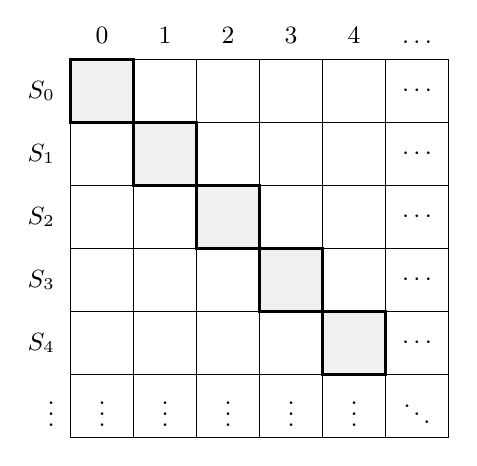
\begin{tikzpicture}[
    every node/.style={font=\small,inner sep=0pt,outer sep=0pt},
    cell/.style ={draw,line width=.4pt,minimum size=8mm,inner sep=0pt},
    tick/.style ={font=\normalsize,green!50!black},
    cross/.style={font=\normalsize,red!70!black}
]

\def\N{4}                      % rows/cols 0…4 are shown explicitly
\pgfmathtruncatemacro\NN{\N+1} % dotted row/column index (=5)

\pgfmathsetseed{15345}         % <- change to get a different random pattern

% ---------------- diagonal box shading (drawn first) ----------------
\foreach \k in {0,...,\N}{
   \fill[black!6] (0.8*\k-0.4,-0.8*\k-0.4) rectangle (0.8*\k+0.4,-0.8*\k+0.4);
}

% ---------------- grid, labels, membership marks ----------------
\foreach \row in {0,...,\NN}{
  \foreach \col in {0,...,\NN}{

      \coordinate (p) at (\col*0.8,-\row*0.8);

      % node name c<row>_<col>
      \node[cell] (c\row_\col) at (p) {};

      % bottom row / rightmost column show dots -----------------
      \ifnum\row=\NN
           \ifnum\col=\NN  \node at (p) {$\ddots$};
           \else           \node at (p) {$\vdots$}; \fi
      \else
           \ifnum\col=\NN  \node at (p) {$\cdots$};
           \else
              % pseudo-random membership mark -------------------
              \pgfmathrandominteger{\rand}{0}{1}
              \ifnum\rand=1
                   \node[tick]  at (p) {\cmark};
              \else \node[cross] at (p) {\xmark}; \fi
           \fi
      \fi
  }
}

% row labels  s_0 … s_N, ⋮
\foreach \row in {0,...,\N}{
   \node[left=2mm] at (c\row_0.west) {$S_{\row}$};
}
\node[left=2mm] at (c\NN_0.west) {$\vdots$};

% column labels 0 … N, …
\foreach \col in {0,...,\N}{
   \node[above=2mm] at (c0_\col.north) {\col};
}
\node[above=2mm] at (c0_\NN.north) {$\dots$};

% bold diagonal boxes
\foreach \k in {0,...,\N}{
   \draw[thick]
         (c\k_\k.north west) rectangle (c\k_\k.south east);
}

\end{tikzpicture}


\end{center}

Each row represents a set of natural numbers.
Each column stands for a number.
A checkmark indicates that the number is in the set,
a cross that it is not.
(So $0$ is in $S_0$, $1$ is not in $S_0$, 2 is not in $S_{0}$, and so on.)
Cantor's method now looks at the diagonal, in bold.
It defines the new set $D$ by \emph{inverting} the diagonal,
swapping crosses and checkmarks.
In the picture,
the inverted diagonal would begin with \xmarkd \cmarkd \xmarkd \xmarkd \cmarkd \ldots,
meaning that $D$ does not contain $0$,
does contain 1,
does not contain 2 and 3,
does contain 4,
and so on.
The so-defined set $D$ is called the \emph{antidiagonal} of the grid.
It can't be anywhere in the list.
And so there can be no list of all sets of natural numbers.

Theorem \ref{thm:cantor} can be strengthened:

\begin{theorem}{Cantor's Theorem (general version)}{cantor}
  For any set $A$,
  the set of subsets of $A$ has strictly greater cardinality than $A$.
\end{theorem}

\begin{proof}
  \emph{Proof}.
  The proof proceeds essentially as before.
  Suppose for reductio that there is a bijection $f: A \to \mathcal{P}(A)$,
  where $\mathcal{P}(A)$ (called the \emph{power set} of $A$)
  is the set of all subsets of $A$.
  Define the antidiagonal set $D$ as
  the set of all members $X$ of $A$ such that $X$ is not in $f(X)$
  -- for short: $D = \{ X \in A : X \notin f(X) \}$.
  Since $D$ is a subset of $A$,
  it is in $\mathcal{P}(A)$.
  But it can't be an output of $f$.
  For suppose it is.
  That is,
  suppose $D = f(X)$ for some $X \in A$.
  Either $X$ is in $D$ or not.
  If $X$ is in $D$,
  then by definition of $D$,
  $X$ is not in $f(X)$.
  But $f(X) = D$,
  so this is impossible.
  If $X$ is not in $D$,
  then by definition of $D$,
  $X$ is in $f(X)$.
  Again, this is impossible.
  \qed
\end{proof}

% Applied to the natural numbers, Cantor's theorem shows that $\mathcal{P}(\mathbb{N})$
% -- the set of all subsets of natural numbers --
% is uncountably infinite.
% Its cardinality is denoted $2^{\aleph_0}$ or $\mathfrak{c}$ (the cardinality of the continuum).
% In fact, $\mathcal{P}(\mathbb{N})$ is equinumerous with the real numbers $\mathbb{R}$.

Cantor's theorem reveals a hierarchy of infinities.
Starting with $\mathbb{N}$,
we can produce larger and larger infinities by taking power sets:
$\mathcal{P}(\mathbb{N})$ is larger than $\mathbb{N}$,
$\mathcal{P}(\mathcal{P}(\mathbb{N}))$ is even larger,
$\mathcal{P}(\mathcal{P}(\mathcal{P}(\mathbb{N})))$ is larger than that,
and so on,
without end.
There are infinitely many infinite cardinals.

% (We have just learned that ``infinitely many'' is not a precise answer.
% Are there \emph{countably many} infinities -- that is, $\aleph_{0}$?
% Or $\aleph_{1}$?
% Or what?
% According to modern set theory,
% the number of infinities is so large that
% it is not measured by any cardinality.)

\begin{exercise}
  Show that if $A$ and $B$ are countably infinite sets, then their union $A \cup B$ is countably infinite.
\end{exercise}

% \begin{exercise}
%   Show that the set of finite subsets of $\mathbb{N}$ is countably infinite.
% \end{exercise}

\begin{exercise}
  Show that if a first-order language has countably many non-logical symbols,
  then the set of all sentences of the language is countably infinite.
\end{exercise}

\section{Planning the completeness proof}

In section \ref{sec:prop-completeness},
we showed that all valid sentences in propositional logic
are derivable from the axiom schemata A1--A3 by Modus Ponens.
This particular result wasn't easy to foresee,
but it wasn't a surprise that
there is \emph{some} mechanical way of checking if
a sentence of propositional logic is valid.
Models of propositional logic are essentially finitary.
A model is a truth-value assignment to the sentence letters.
Since each sentence of propositional logic is composed of finitely many sentence letters,
and there are only finitely many ways of assigning truth-values to these sentence letters,
it is to be expected that
there is a finitary algorithm for deciding whether all
of these assignments make the sentence true.
% (or whether all of them make the sentence true
% if they make some other sentences true).

% Of course,
% it's not too surprising that the precise proof system I've introduced is sound and complete.
% The axioms and rules were chosen with an eye to completeness.
% This is unlike the situation in some nonclassical logics,
% like intuitionistic logic,
% were the proof-theoretic angle takes priority
% and models are defined so that
% the desired proof system comes out sound and complete.
% Hamkins pp.183ff.

In first-order logic,
the situation is very different.
A first-order model consists of an arbitrary set $D$
together with an interpretation of the non-logical vocabulary,
where, for example, every subset of $D$ is a possible interpretation of any monadic predicate.
Even if $D$ itself is countable,
this means that there are usually uncountably many models with that domain.
And $D$ doesn't have to be countable.
It can have any cardinality whatsoever.
The space of first-order models is enormous.
Their number is vastly greater than $\aleph_0$.
There is, in fact, no aleph big enough to measure the number of first-order models.
It is therefore astonishing that
there is a finitary, mechanical method
-- a proof system --
by which one can find every sentence
that is true across the realm of all first-order models.
Astonishing, but true,
as Kurt Gödel showed in 1929.

Gödel's completeness theorem
(not to be confused with his \emph{incompleteness} theorems
that we'll discuss in later chapters)
is noteworthy for other reasons as well.
For example,
it supports the conjecture
that all intuitively valid mathematical arguments can be formalized
as deductions in the first-order calculus.
Let's take for granted, for the sake of the argument, that
every mathematical statement can be expressed in a first-order language.
Now suppose some mathematical argument \emph{can't} be replicated in the first-order calculus.
By the completeness theorem,
it follows that
there is a model in which the premises are true but the conclusion false.
This strongly suggests that the argument wasn't valid.
We'll meet further applications of the completeness theorem later.
First we need to prove it.
% BBJ 185

\iffalse

Also,
suppose I like the number 1, the number 2, the number 3, etc.
It follows model-theoretically that I like all numbers.
But proofs are finite.
So you can't prove the conclusion from the premises.
Yet we have completeness for FOL!

What about the numbers argument?
This argument isn't \textit{logically} valid.
It's \textit{arithmetically} valid, we might say:
valid given the standard meaning of the arithmetical terms.
Arithmetical entailment is not mirrored by any finite proof system!

Completeness entails that all (first-order) logical truths are provable.
Obviously, not all truths are logical truths.
So completeness doesn't mean that all truths are provable.

\fi

% \begin{exercise}
% Which, if any, of these statements are correct? (1) The soundness theorem implies that every sentence provable from the Peano axioms is a true sentence of arithmetic; (2) The completeness theorem implies that every true sentence of arithmetic is provable from the Peano axioms. [yes/no]
% \end{exercise}

Our proof will follow Henkin's 1949 method,
which we used in chapter~\ref{ch:propcal} to prove
the completeness of propositional logic.
Let's recall the key steps.

We want to show that
whenever a sentence $A$ is entailed by a set of sentences $\Gamma$
(meaning that every model that makes all members of $\Gamma$ true also makes $A$ true),
then there is a deduction of $A$ from $\Gamma$.
For short:
if $\Gamma \entails A$ then $\Gamma \vdash A$.
The proof is by contraposition.
We assume $\Gamma \not\vdash A$ and derive $\Gamma \not\entails A$,
as follows.

\begin{cenumerate}
\item Assume $\Gamma \not\vdash A$.
\item Infer that $\Gamma \cup \{ \neg A \}$ is consistent.
\item Show that $\Gamma \cup \{ \neg A \}$ can be extended to a maximal consistent set $\Gamma^{+}$.
\item Construct a model $\Mod{M}$ based on $\Gamma^{+}$ in which all members of $\Gamma^{+}$ are true.
\item Infer that $\Gamma \not\entails A$.
\end{cenumerate}
%
% Why this fails for SOL: https://math.stackexchange.com/questions/4913675/how-completeness-fails-in-second-order-logic
%
As in chapter 1,
we call a set of sentences \emph{consistent}
if no contradiction can be derived from it.
That is,
$\Gamma$ is consistent iff
there is no sentence $A$ such that $\Gamma \vdash A$ and $\Gamma \vdash \neg A$.
Equivalently
(as you showed in exercise \ref{ex:inconsistency};
the proof carries over from propositional logic),
$\Gamma$ is consistent iff
$\Gamma \not\vdash \bot$.

Steps 2 and 5 are easy.
The following lemma establishes step 2,
and is proved just as its propositional counterpart,
lemma \ref{lem:consistency-lemma}.

\begin{lemma}{}{negation-consistency1}
  $\Gamma \not\vdash A$ iff $\Gamma \cup \{\neg A\}$ is consistent.
\end{lemma}
\begin{proof}
  \emph{Proof.}
  Suppose $\Gamma \cup \{\neg A\}$ is inconsistent.
  Then $\Gamma \vdash \neg \neg A$ by RAA
  and so $\Gamma \vdash A$ by DNE.
  Contraposing,
  this means that if $\Gamma \not\vdash A$ then $\Gamma \cup \{ \neg A \}$ is consistent.
  Conversely,
  suppose $\Gamma \vdash A$.
  Then $\Gamma, \neg A \vdash A$ by Mon
  and $\Gamma, \neg A \vdash \neg A$ by Mon and Id.
  So $\Gamma \cup \{ \neg A \}$ is inconsistent. \qed
\end{proof}

It remains to fill in steps 3 and 4:
we need to show that
\emph{every consistent set of sentences is satisfiable}.

Here is the plan.
Let $\Gamma$ be a consistent set of sentences in some first-order language $\L$
(with identity and function symbols).
We'll show how one can construct a model $\Mod{M}$
in which all members of $\Gamma$ are true.
As in chapter \ref{ch:propcal},
we first extend $\Gamma$ to a maximal consistent set $\Gamma^{+}$
that will guide the construction of the model.
For example,
if $\Gamma$ contains $Fa \lor Gb$,
it's not obvious if
our model should satisfy $Fa$ or $Gb$ or both.
$\Gamma^{+}$ will directly contain $Fa$ or $Gb$ or both,
so it answer this question.

Suppose we have $Fa$ in $\Gamma^{+}$.
Our model $\Mod{M}$ must then contain an object $\llbracket a\rrbracket^{\Mod{M}}$ denoted by $a$ that falls in the extension $\llbracket F \rrbracket^{\Mod{M}}$ of $F$.
The nature of the object $\llbracket a\rrbracket^{\Mod{M}}$ is irrelevant.
It proves useful to choose \emph{the individual constant} $a$ as the object denoted by $a$.
Then we can say
that the extension of $F$ comprises all individual constants $c$ for which $Fc \in \Gamma^{+}$.
(It might seem odd to have a model whose domain consists of individual constants,
and in which each constant denotes itself.
But nothing in the definition of a first-order model prevents us from doing this.)

Unfortunately,
there are some complications.
Suppose $\Gamma$ contains $\exists x Fx$.
(Which is short for $\neg \forall x \neg Fx$.)
We want this sentence to be true in our model $\Mod{M}$.
So there must be some object in $\llbracket F \rrbracket^{\Mod{M}}$.
But if $\llbracket F \rrbracket^{\Mod{M}}$ is defined as the set of individual constants $c$ for which $Fc \in \Gamma^{+}$,
there might be no such object,
as there might be no constant $c$ for which $Fc \in \Gamma^{+}$.
We need to ensure that this doesn't happen.
That is,
we need to ensure that
for each existential sentence $\exists x Fx$ in $\Gamma^{+}$,
there is a ``witnessing'' sentence $Fc$ in $\Gamma^{+}$.
The problem is that
$\Gamma$ may already contain $\neg Fc$ for every individual constant $c$.
Then we can't add the required witness without making $\Gamma$ inconsistent.

To get around this problem,
we'll construct $\Gamma^{+}$ in an extend language $\L^{+}$
that adds new individual constants to $\L$.
We can use these constants to ensure that
every existential sentence in $\Gamma$ has a witness.

Another complication arises from the presence of the identity symbol.
If we let each individual constant denote itself,
any identity statement involving different individual constants will be false.
After all,
no constant is identical to any other constant.
But $a=b$ is consistent,
and might be in $\Gamma$ and therefore in $\Gamma^{+}$.
So we'll actually let each constant denote a \emph{set} of terms:
the constant $a$ will denote the set of closed terms $t$ for which
$a=t$ is in $\Gamma^{+}$.
% We can't just use sets of terms,
% because we need to interpret f for all possible inputs,
% even if there's no constant c for which f(a)=c is in the Henkin set.

Let's fill in the details.

\section{The completeness proof}

We'll show that every consistent set of first-order sentences is satisfiable.
As we've seen above
(and as we'll spell out again below),
from this it is only a small step to the completeness theorem.

So let $\Gamma$ be a consistent set of sentences in a first-order language $\L$.
Let $\L^{+}$ be an extension of $\L$ with (countably) infinitely many new individual constants.
We'll extend $\Gamma$ to a maximal consistent set in $\L^{+}$.
First,
though,
we need to confirm that
$\Gamma$ itself is still consistent in the extended language $\L^{+}$.
Consistency is language-relative because
the language determines which instances of the axioms are available.
As we switch from $\L$ to $\L^{+}$,
new axioms become available.
We need to confirm that
these new axioms don't allow deriving a contradiction from $\Gamma$.

\begin{lemma}{}{consistency-in-Lplus}
  If $\Gamma$ is a set of $\L$-sentences that is consistent within $\L$,
  and $\L^{+}$ extends $\L$ by a set of new individual constants,
  then $\Gamma$ is consistent within $\L^{+}$.
\end{lemma}

\begin{proof}
  \emph{Proof} by contraposition.
  Assume that $\Gamma$ is inconsistent within $\L^{+}$.
  Then there is a deduction $A_{1},\ldots,A_{n}$ of $\bot$ from $\Gamma$,
  where each $A_{i}$ is an $\L^{+}$-sentence.
  Being finite,
  the deduction only uses finitely many of the new constants:
  call them $c_{1},\ldots,c_{k}$.
  The deduction also can't use more than finitely many of the old constants in $\L$.
  Since first-order languages have infinitely many constants,
  we can choose $k$ distinct constants $d_{1},\ldots,d_{k}$ from $\L$
  that don't occur in the deduction.
  Now consider the sequence of sentences $A_{1}',\ldots,A_{n}'$ that results from
  $A_{1},\ldots,A_{n}$ by replacing each $c_{i}$ by $d_{i}$.
  It is easy to see that
  \begin{enumerate*}
    \item[(i)] if $A_{i}$ is an axiom then so is $A_{i}'$;
    \item[(ii)] if $A_{i} \in \Gamma$ then $A_{i}' \in \Gamma$
      (sentences in $\Gamma$ don't contain any new constants);
    \item[(iii)] if $A_{i}$ follows from $A_{1},\ldots,A_{i-1}$ by MP or Gen,
      then $A_{i}'$ follows from $A_{1}',\ldots,A_{i-1}'$ by MP or Gen.
  \end{enumerate*}
  So $A_{1}',\ldots,A_{n}'$ is a deduction of $\bot$ from $\Gamma$,
  showing that $\Gamma$ is inconsistent within $\L$.
  \qed
\end{proof}

Next,
we show that
$\Gamma$ can be extended to a maximal consistent set $\Gamma^{+}$ in which
every existential sentence $\exists x A$ has a witness $A(x/c)$.
Such sets are called \emph{Henkin sets}.

\begin{definition}{}{henkin-set}
  A set of sentences $\Gamma$ in a first-order language $\L$ is a \emph{Henkin set in $\L$} if it satisfies the following conditions.
  \begin{cenumerate}
    \item[(i)] $\Gamma$ is consistent (within $\L$).
    \item[(ii)] For every $\L$-sentence $A$, either $A \in \Gamma$ or $\neg A \in \Gamma$. (Maximality)
    \item[(iii)] Whenever $\Gamma$ contains a sentence of the form $\neg \forall x A$
    then it also contains $\neg A(x/c)$ for some individual constant $c$. (Witnessing)
  \end{cenumerate}
\end{definition}
\noindent%
In the presence of the other conditions,
(iii) is equivalent to the requirement that
if $\Gamma$ contains $\neg \forall x \neg A$
then it contains $A(x/c)$ for some $c$.

\begin{exercise}\label{ex:henkin-closure}
  Show that if $\Gamma$ is a Henkin set and $\Gamma \vdash A$, then $A \in \Gamma$.
  % Proof exactly as for lem:max-cons-closure.
\end{exercise}

\begin{exercise}\label{ex:henkin-terms-constants}
  Show that if $\Gamma$ is a Henkin set (in a first-order language with identity) then
  for every closed term $t$ of the language
  there is an individual constant $c$ such that $t=c$ is in $\Gamma$.
  % t=t entails ∃x(x=t). Witnessing requires x=c.
\end{exercise}

\begin{exercise}\label{ex:henkin-quantifiers-prf}
  Show that if $\Gamma$ is a Henkin set then
  $\Gamma$ contains $\forall x A$ iff
  $\Gamma$ contains $A(x/c)$ for every individual constant $c$.
\end{exercise}

\begin{lemma}{}{henkin-extension}
  Every consistent set of $\L$-sentences $\Gamma$ can be extended
  to a Henkin set $\Gamma^+$ in any language $\L^{+}$ that adds infinitely many individual constants to $\L$.
\end{lemma}

\begin{proof}
  \emph{Proof}.
  Let $\Gamma$ be a consistent set of $\L$-sentences.
  Let $A_{1}, A_{2}, \ldots$ be a list of all $\L^{+}$-formulas with exactly one free variable.
  We define a sequence of sets $\Gamma_{0}, \Gamma_{1}, \ldots$ as follows:
  \begin{align*}
    \Gamma_{0} & := \Gamma \\
    \Gamma_{n+1} & := \Gamma_{n} \cup \{ \neg \forall x A_{n} \to \neg A_{n}(x/c_{n}) \},
  \end{align*}
  where $x$ is the free variable in $A_{n}$ and
  $c_{n}$ is a new $\L^{+}$-constant that does not occur in $\Gamma_{n}$.
  (There must be some such constant because $\L^{+}$ contains infinitely many constants
  that don't occur in $\Gamma$.)
  Let $\Gamma'$ be the union $\bigcup_{n} \Gamma_{n}$ of all sets in this sequence.
  (That is, a sentence $A$ is in $\Gamma'$ iff it is in some $\Gamma_{n}$.)

  % Careful: it's not enough to add witnesses for all existential sentences,
  % or to loop only over the universal sentences in $\L$.
  % E.g., if $\Gamma$ contains ∃x∃yRxy, we'd only get the witness ∃yRay.
  % We also want a witness for that, which isn't in Γ and not even in \L, due to the new constant a.

  We show that $\Gamma'$ is consistent.
  Suppose not.
  Then there is a derivation of $\bot$ from $\Gamma$
  and the ``Henkin sentences'' $\neg \forall x A_{n} \to \neg A_{n}(x/c_{n})$.
  This derivation can use only finitely many of the Henkin sentences.
  So one of the $\Gamma_{n}$ must be inconsistent.
  But we can show by induction on $n$ that each $\Gamma_{n}$ is consistent.

  The base case, for $n=0$, holds by assumption: $\Gamma$ is consistent.

  For the inductive step, assume $\Gamma_{n}$ is consistent and
  suppose for reductio that $\Gamma_{n+1}$ is inconsistent.
  By RAA, we then have
  \begin{gather}
    \Gamma_{n} \proves \neg (\neg\forall x A_{n} \to \neg A_{n}(x/c_{n})). \tag{1}
  \end{gather}
  It's easy to show that
  if $\Gamma_n \proves \neg (A \to B)$ then
  $\Gamma_n \proves A$ and $\Gamma_n \proves \neg B$.
  (Both $\neg (A \to B) \to A$ and $\neg (A \to B) \to \neg B$ are truth-functional tautologies.)
  So (1) implies
  \begin{gather}
    \Gamma_{n} \proves \neg \forall x A_{n}, \text{ and} \tag{2}\\
    \Gamma_{n} \proves \neg\neg A_{n}(x/c_{n}). \tag{3}
  \end{gather}
  From (3), we get $\Gamma_{n} \proves A_{n}(x/c_{n})$ by DNE.
  As $c_{n}$ does not occur in $\Gamma_{n}$,
  Gen yields
  \begin{gather}
    \Gamma_{n} \proves \forall x A_{n}. \tag{4}
  \end{gather}
  (2) and (4) show that $\Gamma_{n}$ is inconsistent,
  which contradicts the induction hypothesis.

  Next, we extend $\Gamma'$ to a maximal consistent set $\Gamma^{+}$.
  The construction follows the proof of Lindenbaum's Lemma (lemma \ref{lem:lindenbaum}).
  Let $S_{1}, S_{2}, \ldots$ be a list of all $\L^{+}$-sentences.
  Starting with $\Gamma'$,
  we define another sequence of sets $\Gamma'_{0}, \Gamma'_{1}, \ldots$:
  \begin{align*}
    \Gamma'_{0} & := \Gamma' \\
    \Gamma'_{n+1} & := \begin{cases}
        \Gamma'_{n} \cup \{ S_{n} \} & \text{if } \Gamma'_{n} \cup \{ S_{n} \} \text{ is consistent,} \\
        \Gamma'_{n} \cup \{ \neg S_{n} \} & \text{otherwise.}
        \end{cases}
  \end{align*}

  We show by induction that each $\Gamma'_{n}$ is consistent.
  The \emph{base case}, for $n=0$, holds because $\Gamma'_0$ is $\Gamma'$,
  which we've just shown to be consistent.
  For the \emph{inductive step},
  assume that a set $\Gamma'_n$ in the list is consistent.
  By lemma \ref{lem:extension-consistency}
  (which only depends on RAA and therefore also holds for the first-order calculus),
  either $\Gamma'_n \cup \{ S_n \}$ or $\Gamma'_n \cup \{ \neg S_n \}$ is consistent.
  If $\Gamma'_n \cup \{ S_n \}$ is consistent,
  then $\Gamma'_{n+1}$ is $\Gamma'_n \cup \{ S_n \}$ (by construction),
  so $\Gamma'_{n+1}$ is consistent.
  If $\Gamma'_n \cup \{ S_n \}$ is not consistent,
  then $\Gamma'_{n+1}$ is $\Gamma'_n \cup \{ \neg S_n \}$,
  so again $\Gamma'_{n+1}$ is consistent.

  Let $\Gamma^{+}$ be the union $\bigcup_{n} \Gamma'_{n}$ of $\Gamma'_{0}, \Gamma'_{1}, \ldots$.
  Evidently, $\Gamma$ is a subset of $\Gamma^{+}$.
  We show that $\Gamma^{+}$ is a Henkin set.

  Maximality holds because for each sentence $S_n$,
  one of $S_n$ or $\neg S_n$ is in $\Gamma'_{n+1}$ and therefore in $\Gamma^{+}$.

  To show consistency,
  suppose that $\Gamma^{+}$ is inconsistent.
  Then there are sentences $A_1,\ldots,A_n$ in $\Gamma^+$ from which $\bot$ is deducible.
  All of these sentences have to occur somewhere on the list $S_1,S_2,\ldots$.
  Let $S_j$ be the first sentence from $S_1,S_2,\ldots$ that occurs after
  all the $A_1,\ldots,A_n$.
  Then all $A_1,\ldots,A_n$ are  in $\Gamma'_j$.
  So $\Gamma'_j$ is inconsistent.
  But we've seen that all of the $\Gamma'_n$ are consistent.

  It remains to show that $\Gamma^{+}$ has the witnessing property:
  whenever $\neg \forall x A$ is in $\Gamma^{+}$ then
  $\Gamma^+$ contains a corresponding sentence $\neg A(x/c)$.
  Let $A$ be any formula in which $x$ is the only free variable.
  By construction,
  $\Gamma'$ contains $\neg \forall x A \to \neg A(x/c)$,
  for some constant $c$.
  Since $\Gamma^{+}$ extends $\Gamma'$,
  it also contains this sentence.
  So if $\Gamma^{+}$ contains $\neg \forall x A$
  then it contains $\neg A(x/c)$,
  by MP and exercise~\ref{ex:henkin-closure}.
  \qed
\end{proof}

Next,
we show how to read off a model from a Henkin set.
The model's domain will consist of sets of closed terms,
so that we can stipulate that
each constant $c$ denotes the set of all terms $t$ for which $c=t$ is in the Henkin set.
Let's have a closer look at these sets.

\begin{definition}{}{equivalence}
  A binary relation $R$ on some domain $D$ is an \emph{equivalence relation} if it is
  \begin{cenumerate}
    \item[(i)] \emph{reflexive}: for every $x \in D$, $x R x$;
    \item[(ii)] \emph{symmetric}: for every $x, y \in D$, if $x R y$ then $y R x$; and
    \item[(iii)] \emph{transitive}: for every $x, y, z \in D$, if $x R y$ and $y R z$ then $x R z$.
  \end{cenumerate}
\end{definition}

\begin{lemma}{}{=equivalence}
  If $\Gamma$ is a Henkin set in a language $\L$ then
  the relation $R$ that holds between $\L$-terms $t,s$ iff $t=s \in \Gamma$ is an equivalence relation.
\end{lemma}
\begin{proof}
  \emph{Proof.}
  By A6, $\proves t=t$.
  So $t=t \in \Gamma$ by exercise~\ref{ex:henkin-closure}.
  Symmetry and transitivity follow similarly from exercise~\ref{ex:identity}.
  \qed
\end{proof}

\begin{wrapfigure}{r}{0.32\textwidth}
  \centering
  \scalebox{0.55}{
  \begin{tikzpicture}[
  >=Stealth,
  dot/.style = {circle, fill, inner sep=1.9pt},
  dir/.style = {->, line width=1.0pt, shorten <=1.2pt, shorten >=1.2pt, draw=gray}
]

% Square domain
\draw[thick] (0,0) rectangle (8,8);

% Dots
\node[dot] (A) at (2.0,5.0) {};
\node[dot] (B) at (4.0,6.5) {};
\node[dot] (C) at (6.4,5.5) {};
\node[dot] (E) at (4.8,4.3) {};
\node[dot] (F) at (2.2,1.4) {};
\node[dot] (G) at (6.2,1.6) {};

% B <-> C
\draw[dir] (B) to[bend left=20] (C);
\draw[dir] (C) to[bend left=20] (B);

% E <-> F
\draw[dir] (E) to[bend left=20] (F);
\draw[dir] (F) to[bend left=20] (E);

% F <-> G
\draw[dir] (F) to[bend left=22] (G);
\draw[dir] (G) to[bend left=22] (F);

% E <-> G
\draw[dir] (E) to[bend right=20] (G);
\draw[dir] (G) to[bend right=20] (E);

% Self-loop arrows at each node (kept, now grey)
\draw[dir, looseness=28, out=150, in=210] (A) to (A);
\draw[dir, looseness=28, out=100, in=160] (B) to (B);
\draw[dir, looseness=28, out=350, in=290] (C) to (C);
\draw[dir, looseness=28, out=130, in=70]  (E) to (E);
\draw[dir, looseness=28, out=300, in=240] (F) to (F);
\draw[dir, looseness=28, out=0,   in=300] (G) to (G);

% Dotted grey partition lines (wavy, to edges), separating the three classes:
% {A}, {B,C}, {E,F,G}. Chosen to avoid crossing arrows.
\coordinate (J) at (3.2,5.6);

% To top edge (between A and B/C)
\draw[densely dotted, very thick, draw=gray]
  (J) .. controls (2.9,5.6) and (2.9,6.9) .. (2.0,8.0);

% To left edge (between A and E/F/G)
\draw[densely dotted, very thick, draw=gray]
  (J) .. controls (2.4,4.9) and (1.4,2.6) .. (0.0,2.1);

% To right edge (between B/C and E/F/G)
\draw[densely dotted, very thick, draw=gray]
  (J) .. controls (4.6,5.1) and (6.5,5.3) .. (8.0,3.2);

\end{tikzpicture}

  }
\end{wrapfigure}

An equivalence relation \emph{partitions} the domain over which it is defined into distinct cells so that
within each cell,
all objects stand in the relation to one another.
These cells are called \emph{equivalence classes}.
If $R$ is an equivalence relation and $x$ an object in the domain,
we write `$[x]_{R}$' for the equivalence class of $R$ that contains $x$.
That is, $[x]_{R} = \{ y \in D \,:\, x R y \}$.
If the relation $R$ is clear from the context,
we may simply write `$[x]$'.

When we're talking about a Henkin set $\Gamma$,
the relevant equivalence relation is the one defined in lemma \ref{lem:=equivalence}.
In what follows,
`$[t]$' therefore denotes the set of all terms $s$ for which $t=s \in \Gamma$.

The model $\Mod{M}$ that we'll construct from a Henkin set $\Gamma$ will have as its domain
the set of all equivalence classes $[t]$,
where $t$ is a closed term in the language of $\Gamma$.
By exercise~\ref{ex:henkin-terms-constants},
$[t]$ always contains an individual constant.
So we can also say that $D$ is the set of all $[c]$
where $c$ is an individual constant in the language of $\Gamma$.

We'll stipulate that
the interpretation function $I$ of $\Mod{M}$
assigns $[c]$ to each constant $c$.
So we'll have $\llbracket c \rrbracket^{\Mod{M}} = [c]$.
We'll extend this to function terms,
so that $\llbracket f(c) \rrbracket^{\Mod{M}} = [f(c)]$.
But we can't \emph{directly} stipulate this,
because interpretation functions don't assign denotations to complex terms.
We have to interpret $f$ as denoting a function on $D$.
By definition~\ref{def:denotation},
The denotation of $f(c)$ is
the denotation of $f$ applied to the denotation of $c$.
Since the denotation of $c$ is $[c]$,
we want the denotation of $f$ to be a function that returns $[f(c)]$ for input $[c]$.
So we'll stipulate that for any one-place function symbol $f$ and constant $c$,
$I(f)$ is the function that maps $[c]$ to $[f(c)]$.
Similarly for many-place function symbols.

This kind of stipulation can go wrong.
Suppose $[c]$ contains two constants $c$ and $d$,
and $[f(c)] \neq [f(d)]$.
Our stipulation would entail that $I(f)$
returns $[f(c)]$ for input $[c]$
and $[f(d)]$ for input $[d]$.
But if $c$ and $d$ are both in $[c]$ then $[c] = [d]$.
And a function can't return two different values for the same input.
We must show that this problem can never arise.

A similar issue arises for the interpretation of predicates.
To ensure that $Ft$ is in $\Gamma$ iff $\Mod{M} \satisfies Ft$,
we'll stipulate that
$I(F)$ is the set of all $[t]$ for which $Ft \in \Gamma$.
This set isn't well-defined if
there are cases where $[t]$ contains two terms $t$ and $s$
for which $Ft \in \Gamma$ but $Fs \notin \Gamma$.

The following lemma shows that neither problem can arise.

\begin{lemma}{}{congruence}
  If $f$ is an $n$-ary function symbol,
  $P$ an $n$-ary predicate symbol,
  and $s_{1}, \ldots, s_{n}, t_{1}, \ldots, t_{n}$ are terms such that
  $[s_{1}] = [t_{1}], \ldots, [s_{n}] = [t_{n}]$,
  then
  \begin{cenumerate}
    \item[(i)] $[f(s_1,\ldots,s_n)] = [f(t_{1},\ldots,t_{n})]$;
    \item[(ii)] $P(s_1,\ldots,s_n) \in \Gamma \; \text{iff} \; P(t_1,\ldots,t_n) \in \Gamma$.
  \end{cenumerate}
\end{lemma}

\begin{proof}
  \emph{Proof.}
  Assume $[s_{i}] = [t_{i}]$, for $i=1,2,\ldots,n$.
  So $\Gamma$ contains $s_{i}\!=\!t_{i}$, for each $i=1,2,\ldots,n$.

  (i).
  By A6 (and exercise~\ref{ex:henkin-closure}),
  $f(s_{1},\ldots,s_{n})=f(s_{1},\ldots,s_{n})$ is in $\Gamma$.
  By $n$ instances of A7 and MP,
  it follows that $f(s_{1},\ldots,s_{n})=f(t_{1},\ldots,t_{n})$ is in $\Gamma$,
  which entails that $[f(s_1,\ldots,s_n)] = [f(t_{1},\ldots,t_{n})]$.

  (ii). Assume $P(s_{1},\ldots,s_{n})$ is in $\Gamma$.
  By $n$ instances of A7 and MP,
  $P(t_{1},\ldots,t_{n})$ is in $\Gamma$ as well.
  The converse holds by the same reasoning.
  \qed
\end{proof}

Lemma \ref{lem:congruence} ensures that the following definition is legitimate.

\begin{definition}{}{henkin-model}
  If $\Gamma$ be a Henkin set in a language $\L$
  then the \emph{Henkin model} $\Mod{M}_{\Gamma}$ of $\Gamma$ is defined as follows.

  The domain $D$ of $\Mod{M}_{\Gamma}$ is the set
  of all $[c]$ where $c$ is an individual constant of $\L$.

  The interpretation function $I$ of $\Mod{M}_{\Gamma}$ maps
  \begin{cenumerate}
    \item[(i)] each individual constant $c$ to $[c]$,
    \item[(ii)] each $n$-ary function symbol $f$ to the function on $D$ that maps
         any $n$ objects $[t_1],\ldots,[t_n]$ to $[f(t_1,\ldots,t_n)]$,
    \item[(iii)] each (non-logical) $n$-ary predicate symbol $P$ to
         the set of all $n$-tuples $\t{[t_1],\ldots,[t_n]}$ such that $P(t_1,\ldots,t_n) \in \Gamma$.
  \end{cenumerate}
\end{definition}

Now remember what we're trying to achieve.
We want to show that
every consistent set of sentences is satisfiable.
We've shown in lemma~\ref{lem:henkin-extension} that
every such set can be extended to a Henkin set.
Definition~\ref{def:henkin-model} tells us
how to construct a model from this Henkin set.
It remains to show that
all members of the Henkin set
(and therefore all members of the original set)
are true in this model.

We'll need the following two facts.

\begin{lemma}{}{henkin-terms}
  If $\Mod{M}$ is a Henkin model and $t$ a closed term then
  $\llbracket t \rrbracket^{\Mod{M}} = [t]$.
\end{lemma}
\begin{proof}
  \emph{Proof}.
  The proof is by induction on complexity of $t$.
  The base case is covered by clause (i) in definition \ref{def:henkin-model}.
  So let $t$ be $f(t_{1},\ldots,t_{n})$.
  Then
  \begin{align*}
    \llbracket f(t_{1},\ldots,t_{n})\rrbracket^{\Mod{M}} &= \llbracket f\rrbracket^{\Mod{M}}(\llbracket t_{1}\rrbracket^{\Mod{M}},\ldots,\llbracket t_{n}\rrbracket^{\Mod{M}}) &&\text{ by def.\ \ref{def:satisfaction=}}\\
                               &= \llbracket f\rrbracket^{\Mod{M}}([t_{1}],\ldots,[t_{n}]) &&\text{ by ind.\ hyp.}\\
                               &= [f(t_{1},\ldots,t_{n})] &&\text{ by def.~\ref{def:henkin-model}.} \qed
  \end{align*}
\end{proof}

\begin{lemma}{}{henkin-quantifiers}
  If $\Mod{M}$ is a Henkin model and $A$ a formula then
  $\Mod{M} \satisfies \forall x A$ iff
  $\Mod{M} \satisfies A(x/c)$ for all individual constants $c$.
\end{lemma}
\begin{proof}
  \emph{Proof.}
  We first show that
  if $\Mod{M}^{d:[c]}$ is a model just like $\Mod{M}$
  except that it assigns $[c]$ to $d$,
  and $d$ does not occur in $A$,
  then
  \begin{equation}\tag{1}
    \Mod{M}^{d:[c]} \satisfies A(x/d)\text{ iff }\Mod{M} \satisfies A(x/c).
  \end{equation}
  There are two cases to consider.
  If $d$ is $c$ then $\Mod{M}^{d:[c]}$ is $\Mod{M}$ and (1) holds trivially.
  If $d$ is a constant other than $c$, then $d$ does not occur in $A(x/c)$.
  So $\Mod{M}^{d:[c]}$ and $\Mod{M}$ agree on the interpretation of all symbols in $A(x/c)$
  and we have
  $\Mod{M}^{d:[c]} \satisfies A(x/c)$ iff $\Mod{M} \satisfies A(x/c)$
  by the coincidence lemma (lemma~\ref{lem:coincidence}).
  Also, by the extensionality lemma (lemma~\ref{lem:extensionality}),
  $\Mod{M}^{d:[c]} \satisfies A(x/d)$ iff $\Mod{M}^{d:[c]} \satisfies A(x/c)$.
  So (1) holds.

  Now, by definition \ref{def:satisfaction=},
  $\Mod{M} \satisfies \forall x A$ iff
  $\Mod{M}' \satisfies A(x/d)$ for every model $\Mod{M}'$
  that differs from $\Mod{M}$ at most in the object assigned to $d$,
  where $d$ is the alphabetically first constant that does not occur in $A$.
  Since each such $\Mod{M}'$ has the same domain as $\Mod{M}$,
  the set of such $\Mod{M}'$ is precisely the set of
  variants $\Mod{M}^{d:[c]}$ of $\Mod{M}$,
  So $\Mod{M} \satisfies \forall x A$ iff
  $\Mod{M}^{d:[c]} \satisfies A(x/d)$ for every constant $c$,
  which, by (1), is the case iff
  $\Mod{M} \satisfies A(x/c)$ for every constant $c$.
  \qed
\end{proof}

\begin{lemma}{Truth Lemma}{truth}
  If $\Mod{M}$ is the Henkin model of a Henkin set $\Gamma$ in a language $\L$,
  then for every $\L$-sentence $A$,
  $\Mod{M} \satisfies A$ iff $A \in \Gamma$.
\end{lemma}

\begin{proof}
  \emph{Proof}
  by induction on  complexity of $A$.

  \emph{Base case}:
  $A$ is atomic. There are two subcases.

  Assume that $A$ is an identity sentence $s=t$.
  Then $\Mod{M} \satisfies s=t$
  iff $\llbracket s\rrbracket^{\Mod{M}} = \llbracket t\rrbracket^{\Mod{M}}$
  by definition \ref{def:satisfaction=},
  iff $[s] = [t]$
  by lemma~\ref{lem:henkin-terms},
  iff $s=t \in \Gamma$,
  by definition of the equivalence classes.

  Assume next that $A$ is an atomic sentence $P(t_{1},\ldots,t_{n})$,
  where $P$ is non-logical.
  Then $\Mod{M} \satisfies P(t_{1},\ldots,t_{n})$
  iff $(\llbracket t_{1}\rrbracket^{\Mod{M}},\ldots,\llbracket t_{n}\rrbracket^{\Mod{M}}) \in \llbracket P\rrbracket^{\Mod{M}}$
  by definition \ref{def:satisfaction=},
  iff $([t_{1}],\ldots,[t_{n}]) \in \llbracket P\rrbracket^{\Mod{M}}$
  by lemma~\ref{lem:henkin-terms},
  iff $P(t_{1},\ldots,t_{n}) \in \Gamma$
  by definition \ref{def:henkin-model}.

  \emph{Inductive step:}
  $A$ is composed of other sentences.
  We have three subcases.
  The first two,
  where $A$ is $\neg B$ or $B \to C$,
  are easy and go exactly as in lemma~\ref{lem:truth-lemma}.
  I'll skip them.

  % Assume that $A$ is a $\neg B$,
  % for some sentence $B$.
  % We need to show that $\Mod{M} \satisfies \neg B$ iff $\neg B \in \Gamma$.
  % Left to Right:
  % Assume $\Mod{M} \satisfies \neg B$.
  % Then $\Mod{M} \not\satisfies B$ by definition \ref{def:satisfaction=}.
  % So $B \notin \Gamma$ by induction hypothesis.
  % So $\neg B \in \Gamma$ by maximality of $\Gamma$.
  % Right to Left:
  % Assume $\neg B \in \Gamma$.
  % Then $B \not\in \Gamma$ by consistency of $\Gamma$.
  % So $\Mod{M} \not\satisfies B$ by induction hypothesis.

  % Assume next that $A$ is $B \to C$,
  % for some sentences $B$ and $C$.
  % We need to show that $\Mod{M} \satisfies B \to C$ iff $B \to C \in \Gamma$.
  % Left to Right:
  % Assume $\Mod{M} \satisfies B \to C$.
  % Then $\Mod{M} \not\satisfies B$ or $\Mod{M} \satisfies C$ by definition \ref{def:satisfaction=}.
  % If $\Mod{M} \not\satisfies B$, then by induction hypothesis $B \notin \Gamma$,
  % so by maximality $\neg B \in \Gamma$.
  % Since $\neg B \proves B \to C$,
  % it follows that $B \to C \in \Gamma$.
  % If $\Mod{M} \satisfies C$, then by induction hypothesis $C \in \Gamma$.
  % Since $C \proves B \to C$,
  % it again follows that $B \to C \in \Gamma$.
  % Right to Left:
  % Assume $B \to C \in \Gamma$.
  % If $B \in \Gamma$, then $C \in \Gamma$ by MP,
  % and by induction hypothesis $\Mod{M} \satisfies C$.
  % By definition \ref{def:satisfaction=}, this means that
  % $\Mod{M} \satisfies B \to C$.
  % If, on the other hand, $B \not\in \Gamma$
  % then by induction hypothesis $\Mod{M} \not\satisfies B$,
  % and $\Mod{M} \satisfies B \to C$ by definition \ref{def:satisfaction=}.

  For the final subcase,
  assume that $A$ is $\forall x B$,
  for some formula $B$.
  We have:
  $\Mod{M} \satisfies \forall x B$ iff
  $\Mod{M} \satisfies B(x/c)$ for every constant $c$ by lemma~\ref{lem:henkin-quantifiers},
  iff $B(x/c) \in \Gamma$ for every constant $c$ by induction hypothesis,
  iff $\forall x B \in \Gamma$ by exercise~\ref{ex:henkin-quantifiers-prf}.
  \qed
\end{proof}

With that,
we have all the ingredients for the completeness proof.

\begin{theorem}{Completeness of the first-order calculus (Gödel 1929)}{completeness}
  If $\Gamma \entails A$ then $\Gamma \proves A$.
\end{theorem}

\begin{proof}
  \emph{Proof.}
  We argue by contraposition.
  Assume $\Gamma \notproves A$.
  Then $\Gamma \cup \{\neg A\}$ is consistent,
  by lemma~\ref{lem:negation-consistency1}.
  By lemma~\ref{lem:henkin-extension},
  $\Gamma \cup \{ \neg A \}$ can be extended to a Henkin set $\Gamma^{+}$ in an extended language $\L^{+}$.
  By the Truth Lemma,
  the Henkin model of $\Gamma^{+}$ satisfies every sentence in $\Gamma^{+}$,
  and therefore every sentence in $\Gamma \cup \{\neg A\}$.
  So there is a model that satisfies all sentences in $\Gamma$ but doesn't satisfy $A$.
  So $\Gamma \not\entails A$. \qed
\end{proof}

Technically,
the model that figures in this proof is not
a model for the original language $\L$ of $\Gamma$ and $A$,
because it also interprets the added individual constants.
If this bothers you,
we can define an $\L$-model that falsifies $\Gamma \entails A$
by restricting the interpretation function of the Henkin model
to $\L$-constants,
without changing the domain.
This is called the \emph{reduct} of the Henkin model to $\L$.

\begin{exercise}
  Assume that $\Gamma_{0}, \Gamma_{1}, \ldots$ are consistent sets of sentences
  in a first-order language $\L$,
  and that each $\Gamma_{i}$ is a subset of $\Gamma_{i+1}$.
  Show that their union $\bigcup_{i} \Gamma_{i}$ is consistent.
\end{exercise}

\section{Unintended Models}
\label{sec:unintended}

We've now shown that the first-order calculus is both sound (theorem~\ref{thm:soundness})
and complete (theorem~\ref{thm:completeness}):
$\Gamma \entails A$ iff $\Gamma \proves A$.
As Gödel pointed out,
this has a curious consequence:

\begin{theorem}{Compactness of first-order logic (Gödel 1929)}{compactness}
   If every finite subset of a set of sentences is satisfiable then the set itself is satisfiable.
\end{theorem}

% The word 'compact', in this use, is inherited from topology,
\begin{proof}
  \emph{Proof.}
  Let $\Gamma$ be a set of first-order sentences.
  Assume that $\Gamma$ is not satisfiable.
  So $\Gamma \entails \bot$.
  By completeness,
  it follows that $\Gamma \proves \bot$:
  there is a deduction of $\bot$ from $\Gamma$.
  This deduction can only use finitely many sentences from $\Gamma$.
  So there is a finite subset $\Gamma'$ of $\Gamma$ for which $\Gamma' \proves \bot$.
  By soundness,
  $\Gamma' \entails \bot$.
  \qed
\end{proof}

% \begin{corollary}{}{}
%   If $\Gamma \entails A$ then
%   there is a finite subset $\Gamma_{0}$ of $\Gamma$ such that $\Gamma_{0} \entails A$.
% \end{corollary}

Why is this curious?
Well, for one,
it is easy to come up with cases where a conclusion is entailed by infinitely many premises,
but not by any finite subset of those premises.
For example,
consider the premises
`I like the number 0',
`I like the number 1',
`I like the number 2',
and so on, for all natural numbers.
Together,
these premises entail `I like all natural numbers'.
But no finite subset of the premises does.
This doesn't contradict the compactness theorem because the inference isn't \emph{logically} valid:
it depends on the interpretation of `0', `1', `2', \ldots, and `natural number'.
Still,
it's curious that first-order logic doesn't allow any such inference to be valid.
More directly,
compactness implies that
there is no way to fully pin down the interpretation of `0', `1', `2', etc.\
in a first-order language.
Let's think through this more carefully.

Many branches of mathematics can be seen as studying certain \emph{mathematical structures}.
A mathematical structure consists of a set of objects together with some operations and relations on these objects.
For example,
arithmetic studies operations and relations on the
natural numbers.
A formalized, first-order theory of arithmetic will have
nonlogical symbols for, say, addition (`$+$'),
multiplication (`$\times$'),
and the less-than relation (`$<$').
We might add an individual constant `$n$' for each number $n$,
but for the sake of economy we can instead have a single constant `0' for 0
and another symbol `$s$' for the successor function
that maps each number $n$ to its successor $n+1$.
Instead of `1', we can then write `$s(0)$';
`2' is `$s(s(0))$', and so on.

In \emph{logic}, we abstract away from the meaning of the nonlogical symbols.
In \emph{arithmetic}, we don't.
In arithmetic, `$1+2=3$'
(that is, `$s(0) + s(s(0)) = s(s(s(0)))$')
is a definite claim about the natural numbers.
We say that it has an \emph{intended interpretation},
or an \emph{intended model}.

The intended model of arithmetic,
also known as the \emph{standard model} of arithmetic, or $\Mod{A}$,
has as its domain
the set of natural numbers $\mathbb{N}$;
it interprets `0' as denoting 0,
`+' as denoting the addition function +,
`$\times$' as denoting the multiplication function $\times$,
`$s$' as denoting the successor function $s$, and
`$<$' as denoting the less-than relation $<$.
We can represent this as a list:
$\t{\mathbb{N}, 0, +, \times, s, <}$.
The list represents the ``structure'' of the natural numbers.
It identifies a set $\mathbb{N}$
and some operations and relations on that set
that are picked out by the nonlogical symbols of the language.
(0 counts as a zero-ary operation.)

Of course,
the language of arithmetic also has unintended models.
For example,
we can let the domain be $\{$ Athens, Berlin $\}$
and use an interpretation function that maps
`0' to Athens,
`+' and `$\times$' to the function that maps any pair of cities to Athens,
`$s$' to the function that maps each city to itself,
and
`<' to the empty relation.
In this model,
`$s(0) + s(s(0)) = s(s(s(0)))$' is true,
but so is `$s(0) = 0$'.

\begin{exercise}
  Is Lagrange's Theorem (every natural number is the sum of four squares) true in this model?
\end{exercise}

We might hope that
such unintended models can always be ruled out
by laying down sufficiently many postulates in the formal language of arithmetic.
For example,
if our theory of arithmetic contains `$s(0) \ne 0$'
then the above model (with Athens and Berlin) is no longer a model of the theory.
So we can rule out \emph{some} unintended models.
The compactness theorem dashes any hope
of ruling out \emph{all} unintended models.
Let $\mathrm{Th}(\Mod{A})$ be the set of all sentences true in
the standard model $\Mod{A}$.
This is called the \emph{theory of $\Mod{A}$}.
It contains all postulates we could possibly lay down,
assuming that they should all be true in the standard model.
By compactness,
there is a model of $\mathrm{Th}(\Mod{A})$ whose domain
includes junk elements that clearly aren't natural numbers.

\begin{theorem}{Non-standard Models of Arithmetic}{non-standard-arithmetic}
  $\mathrm{Th}(\Mod{A})$ has models in which
  some object is not reachable from 0
  by finitely many applications of the successor function.
  (Such models are called \emph{non-standard models} of arithmetic.)
\end{theorem}
\begin{proof}
  \emph{Proof.}
  Let $\L_A^+$ be the language of arithmetic
  with an added individual constant $c$.
  Let $\mathrm{Th}(\Mod{A})^+$ be the set of sentences that
  extends $\mathrm{Th}(\Mod{A})$ by
  \[
    c \ne 0, \quad c \ne s(0), \quad c \ne s(s(0)), \quad c \ne s(s(s(0))), \quad\ldots.
  \]
  So $\mathrm{Th}(\Mod{A})^+$ says that
  $c$ is different from 0, 1, 2, and so on, for all natural numbers.
  Every finite subset of $\mathrm{Th}(\Mod{A})^+$ is obviously satisfiable:
  it is true in the standard model $\Mod{A}$,
  interpreting $c$ as a sufficiently large number.
  By the compactness theorem,
  it follows that $\mathrm{Th}(\Mod{A})^+$ is satisfiable.
  Any model of $\mathrm{Th}(\Mod{A})^+$
  must have an element (denoted by $c$) that
  is not identical to any natural number:
  it can't be reached from 0 by finitely many applications of the successor function.
  The reduct of any such model to the original language of arithmetic
  (discarding the interpretation of $c$)
  is a model of $\mathrm{Th}(\Mod{A})$.
  \qed
\end{proof}

Compactness thus reveals a deep expressive limitation of first-order logic:
the structure of the natural numbers can't be captured in a first-order language.

Here is a simpler example.
For each $n>0$,
it is easy to find a first-order sentence $S_n$ that is true in all and only
the models with exactly $n$ elements.
For example,
$\exists x \exists y (x \ne y \land \forall z (z=x \lor z=y))$
is true in all and only models with exactly two elements.
(Compare exercise~\ref{ex:domain-size}.)
In that sense,
we can capture the intended size of a domain,
as long as that size is a fixed finite number.
But there is no first-order sentence
that is true in all and only
the models with infinitely many elements.

To see why,
let $S_\infty$ be such a sentence.
Its negation $\neg S_\infty$ would be true in all and only
the finite models.
Now consider the set consisting of $\neg S_\infty$ together with
$\neg S_1, \neg S_2, \neg S_3, \ldots$.
All finite subsets of this set are satisfiable.
By compactness,
the whole set is satisfiable.
But there is no model whose domain not infinite,
and yet also has no finite size.

The following theorems show that
the situation is even worse.
In section~\ref{sec:cardinalities},
we saw that there are many levels of infinity:
many infinite cardinalities.
None of them can be captured in first-order logic,
insofar as there is no sentence (nor even a set of sentences) that would
force a model to have a particular infinite cardinality,
or even to fall in any non-trivial range of infinite cardinalities.

\begin{theorem}{The (Downward) Löwenheim-Skolem Theorem}{lowenheim-skolem-down}
  If a set of sentences in a countable first-order language has a model,
  then it has a countable model.
\end{theorem}

\begin{proof}
  \emph{Proof.}
  Let $\Gamma$ be such a set.
  By lemma~\ref{lem:henkin-extension},
  $\Gamma$ can be extended to a Henkin set $\Gamma^{+}$.
  By lemma~\ref{lem:truth},
  the Henkin model of $\Gamma^{+}$ is a model of $\Gamma$.
  Its domain consists of equivalence classes of closed terms in the language of $\Gamma^{+}$.
  If the language of $\Gamma$ is countable,
  then so is the language of $\Gamma^{+}$.
  So it has only countably many closed terms.
  \qed
\end{proof}

\begin{theorem}{The Upward Löwenheim-Skolem Theorem (Tarski 1935)}{lowenheim-skolem-up}
  If a set of sentences in a countable first-order language has an infinite model,
  then it has models of every infinite cardinality.
\end{theorem}

\begin{proof}
  \emph{Proof sketch.}
  The proof requires relaxing our stipulation that
  a first-order language must only have countably many individual constants.
  The completeness theorem can be proved without this assumption
  (although the proof becomes more complicated,
  as we can no longer appeal to enumerations of the sentences in the language).
  Compactness still follows from completeness,
  and we get a slightly generalized downward Löwenheim-Skolem theorem
  according to which every satisfiable set of sentences has a model
  whose cardinality is at most equal to the cardinality of the language.

  Now let $\Gamma$ be a set of first-order sentences in a countable language
  with an infinite model.
  From the downward theorem,
  we know that $\Gamma$ has a countably infinite model $\Mod{M}$.
  Let $\kappa$ be any cardinal greater than $\aleph_0$.
  Expand the language of $\Gamma$ by $\kappa$ new individual constants.
  For each pair of these constants $c_{i}$ and $c_{j}$,
  add the sentence $c_{i} \neq c_{j}$ to $\Gamma$,
  thereby creating the set $\Gamma^{+}$.
  All finite subsets of $\Gamma^{+}$ are satisfied in $\Mod{M}$,
  with the (finitely many) new constants in the set interpreted as distinct objects in $\Mod{M}$.
  By the compactness theorem (for uncountable languages),
  $\Gamma^{+}$ has a model $\Mod{M}^{+}$.
  All the $\kappa$ new constants denote distinct objects in this model,
  so $\Mod{M}^+$ has at least $\kappa$ objects.
  By the generalized downward theorem,
  it follows that $\Gamma^{+}$ has a model whose cardinality is exactly $\kappa$.
  The reduct of that model to the language of $\Gamma$ is a model of $\Gamma$ with cardinality $\kappa$.
  \qed
\end{proof}

The downward theorem was proved by Thoralf Skolem in 1920,
building on an earlier proof sketch by Leopold Löwenheim.
The (ill-named) upward theorem,
due to Alfred Tarski,
requires compactness and could only be proved after 1929.
It entails,
among other things,
that $\mathrm{Th}(\Mod{A})$ has non-standard models of every infinite cardinality.

\begin{exercise}
  (a) Can you find a first-order sentence that is only true in infinite models?
  (Hint: let $f$ be a function that is injective, but not surjective.)
  (b) Is the negation of this sentence only true in finite models?
\end{exercise}

\begin{exercise}
  Explain why every satisfiable set of first-order sentences has a model whose
  domain is a set of natural numbers.
\end{exercise}

\begin{exercise}
  Consider a first-order language with a binary predicate symbol `$P$' for the ``parent'' relation,
  so that $Pxy$ means (on its intended interpretation) that $x$ is a parent of $y$.
  We can then define the ``grandparent'' relation $P^2(x,y)$ as $\exists z_1 (Pxz_1 \land Pz_1y)$,
  the ``great-grandparent'' relation $P^3(x,y)$ as $\exists z_1 \exists z_2 (Pxz_1 \land Pz_1z_2 \land Pz_2y)$,
  and so on.
  Show that there is no way to define the ``ancestor'' relation
  (no matter what other nonlogical symbols we add to the language):
  there can be no formula $A(x,y)$ that is equivalent to the infinite disjunction
  $P(x,y) \lor P^2(x,y) \lor P^3(x,y) \lor \ldots$.
\end{exercise}

\begin{exercise}
  Let $\Mod{A}^{c}$ be exactly like the standard model of arithmetic $\Mod{A}$,
  except that the number 2 is replaced by Julius Caesar:
  the domain of $\Mod{A}^c$ is $\{ 0, 1, \text{Caesar}, 3, 4, \ldots \}$;
  '$s$' denotes a function that maps 0 to 1, 1 to Caesar, Caesar to 3, \ldots;
  `$+$' denotes a function that maps 1 and 1 to Caesar, 1 and Caesar to 3,
  and so on.
  Is $\Mod{A}^{c}$ a model of $\mathrm{Th}(\Mod{A})$?
  In what way is it less interesting than the non-standard models of theorem~\ref{thm:non-standard-arithmetic}?
\end{exercise}

% This model satisfies all sentences in $\mathrm{Th}(\Mod{A})$,
% and it isn't the intended model.
% Unlike the non-standard models of theorem~\ref{thm:non-standard-arithmetic},
% however,
% this model has the same abstract structure as the standard model:
% the models are \emph{isomorphic},
% meaning that
% there is a one-to-one correspondence between the objects in their domains
% that preserves the operations and relations (in both directions).
% Many mathematicians hold that mathematics is really the study of these more abstract structures:
% the kind of structure that $\Mod{A}$ and $\Mod{M}^{jc}$ have in common.
% (This is called \emph{structuralism} in the philosophy of mathematics.)

% \begin{exercise}
%   A relation $\preceq$ on a set $D$ is a \emph{linear order} if it is
%   \begin{cenumerate}
%     \item[(i)] \emph{reflexive}: for every $x$ in $D$, $x \preceq x$;
%     \item[(ii)] \emph{transitive}: if $x \preceq y$ and $y \preceq z$ then $x \preceq z$;
%     \item[(iii)] \emph{anti-symmetric}: if $x \preceq y$ and $y \preceq x$ then $x=y$;
%     \item[(iv)] \emph{total}: for every $x,y$ in $D$, either $x \preceq y$ or $y \preceq x$.
%   \end{cenumerate}
%   These conditions are easily translated into a first-order language
%   So we can capture the concept of a linear order in first-order logic:
%   we can find a set of first-order sentences with a predicate symbol `$\preceq$'
%   that is true in a model iff the model interprets `$\preceq$' as a linear order.

%   A linear order $\preceq$ is a \emph{well-order} if
%   every non-empty subset of $D$ has a $\preceq$-least element.
%   That is,
%   every non-empty subset $S$ of $D$ has some element $x \in S$ such that
%   for every $y \in S$, $x \preceq y$.
%   For example,
%   the less-than-or-equal relation $\leq$ on the natural numbers $\mathbb{N}$ is a well-order:
%   any set of natural numbers has a least element.
%   Show that
%   the concept of a well-order cannot be captured in first-order logic:
%   there is no set of first-order sentences with a predicate symbol `$\preceq$'
%   that is true in a model iff the model interprets `$\preceq$' as a well-order.
% \end{exercise}

% Suppose for reductio that some set of first-order sentences $\Gamma$
% is true in a model iff it interprets `$\preceq$' as a well-order.
% In particular,
% $\Gamma$ is true in the model $M$ whose domain are the natural numbers $\mathbb{N}$ and
% that interprets `$\preceq$' as the less-than-or-equal relation on $\mathbb{N}$.
% Now let $c_{1},c_{2},\ldots$ be a list of individual constants.
% Construct an extension $\Gamma^{+}$ of $\Gamma$ by adding,
% for each $c_{i}$,
% the sentence
% \[
%   c_{i+1} \preceq c_{i} \land c_{i+1} \not= c_{i},
% \]
% which we may abbreviate as
% \[
%   c_{i+1} \prec c_{i}.
% \]
% Every finite subset of $\Gamma^{+}$ is still satisfiable:
% it is true in the model $M$ just mentioned.
% By compactness, $\Gamma^{+}$ has a model.
% But that model must have an infinite descending chain $\ldots c_{i+1} \prec c_{i} \ldots \prec c_{1}$.
% So it is not a well-order.

% Compactness is a fundamental theorem in model theory.
% Like Gödel,
% we've derived it from completeness,
% but note that it has nothing to do with proofs.
% It's a purely model-theoretic result,
% that can also be proved without any reference to proofs.

% In fact,
% we can use a version of our Henkin proof of Completeness.
% Call a set $\Gamma$ \emph{finitely satisfiable} if every finite subset of $\Gamma$ is satisfiable.
% Assume that $\Gamma$ is finitely satisfiable.
% We would show that $\Gamma$ can be extended to a maximal finitely satisfiable set $\Gamma^{+}$
% in a language $\L^{+}$ with new constant symbols.
% The Henkin model of $\Gamma^{+}$ is then a model of $\Gamma$.


% \begin{exercise}
%   A proof system $\proves$ is called \emph{weakly complete} if it can prove all validities:
%   if $\entails A$ then $\proves A$.
%   In the previous section,
%   we've shown that first-order logic is \emph{strongly complete}:
%   if $\Gamma \entails A$ then $\Gamma \proves A$.
%   Strong completeness obviously implies weak completeness.
%   We've seen that it also implies compactness.
%   Show that, conversely, weak completeness and compactness together imply strong completeness,
%   given that $\proves$ has the standard structural properties and MP.

%   % Answer:
%   % Suppose Γ ⊨ φ.
%   % So Γ ∪ {¬φ} is unsatisfiable.
%   % By compactness, some finite Γ₀ ⊆ Γ makes Γ₀ ∪ {¬φ} unsatisfiable.
%   % Let ψ be the conjunction of the formulas in Γ₀. Unsatisfiability of Γ₀ ∪ {¬φ} is the same as validity of ψ → φ. Hence ⊨ ψ → φ.
%   % By weak completeness, ⊢ ψ → φ.
%   % By Id and Mon, Γ ⊢ ψ. [????]
%   % So by MP, Γ ⊢ φ.
% \end{exercise}

% \begin{exercise}
%   Compactness is an immediate consequence of Completeness.
%   Can you argue in the other direction from Compactness to Completeness?
% \end{exercise}



\iffalse

Let's think about what these theorems mean,
starting with compactness.
It is easy to find cases where
a conclusion is entailed by infinitely many premises,
but not by any finite subset of those premises.
For example,
from the premises:

\begin{quote}
  I like the number 0;\\
  I like the number 1;\\
  I like the number 2;\\
  \ldots
\end{quote}

and so on, for all natural numbers,
one can infer

\begin{quote}
  I like all natural numbers.
\end{quote}

But this conclusion is not entailed by any finite subset of the premises.
Similarly,
one can infer that
some person X is not an ancestor of some person Y
from the assumptions that

\begin{quote}
  X is not a parent of Y;\\
  X is not a parent of a parent of Y;\\
  X is not a parent of a parent of a parent of Y;\\
  \ldots
\end{quote}

and so on, but not from any finite subset of those assumptions.

The compactness theorem shows that
this kind of situation never arises for \emph{first-order logical entailment}.
The two inference just describe are valid,
but their validity depends on the meaning of non-logical terms:
`1', `2', `3', \ldots, and `number' in the first case;
`parent' and `ancestor' in the second.
From the compactness of first-order logic,
it immediately follows that
one can't define these concepts
using only the connectives, the first-order quantifiers, and identity.

What if we declare the relevant terms to be logical?
Let's see what this would mean for a formalized version of the first inference.
Take a first-order language
with infinitely many constants `0', `1', `2', \ldots, and predicate symbols `$N$' and `$L$'.
The premises can then be formulated as: $L0$, $L1$, $L2$, \ldots.
The conclusion is: $\forall x (Nx \to Lx)$.
Obviously,
the conclusion is not entailed by the premises in the ordinary sense of first-order logical entailment:
we can easily find an interpretation of `0', `1', `2', \ldots, `N', and `L'
that makes the premises true and the conclusion false.
But now the idea is that we can define a new kind of entailment
-- call it ``arithmetical entailment'' --
by fixing the interpretation of the `0', `1', `2', \ldots, and `$N$':
`0' must denote the number zero,
`1' the number one, \ldots,
and the extension of `$N$' must be the set of natural numbers.
Some premises $\Gamma$ ``arithmetically entail'' a conclusion $A$ if
any model of $\Gamma$ that conforms to these rules is a model of $A$.
Now $\{ L1, L2, \ldots \}$ arithmetically entails $\forall x (Nx \to Lx)$.
But no finite subset of $\{ L0, L1, \ldots \}$ arithmetically entails $\forall x (Nx \to Lx)$.
So arithmetical entailment is not compact.
Since compactness is a consequence of soundness and completeness,
it follows that
there can't be a sound and complete proof system for arithmetical validity.
That is,
there is no way to spell out axioms and rules of inference that define a proof relation $\proves_{\Mod{A}}$ so that
$\Gamma \proves_{\Mod{A}} A$ iff $\Gamma$ arithmetically entails $A$
-- as long as proofs remain finite.

\begin{exercise}
  Explain how the argument can be run with a single non-arithmetical constant $c$ instead of the predicate symbol $L$.
\end{exercise}

\fi


%%% Local Variables:
%%% mode: latex
%%% TeX-master: "logic3.tex"
%%% End:
